\documentclass[12pt]{article}
\usepackage{amsmath,amssymb}
\usepackage{tikz}
\usepackage{tkz-tab}
\begin{document}
Bảng biến thiên nhiều dòng:

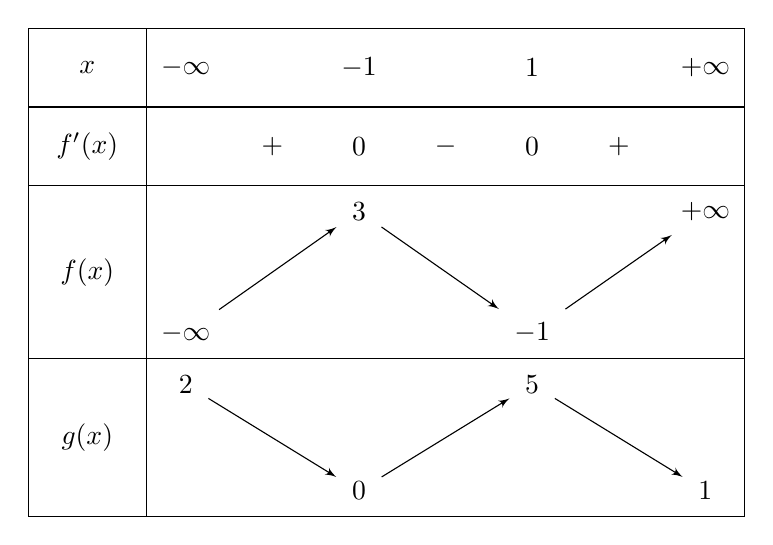
\begin{tikzpicture}
\tkzTabInit[lgt=1.5,espcl=2.2]{$x$ /1, $f'(x)$ /1, $f(x)$ /2.2, $g(x)$ /2}{$-\infty$, $-1$, $1$, $+\infty$}
\tkzTabLine{ , +, 0, -, 0, + , }
\tkzTabVar{-/ $-\infty$, +/ $3$, -/ $-1$, +/ $+\infty$}
\tkzTabVar{+/ $2$, -/ $0$, +/ $5$, -/ $1$}
\end{tikzpicture}

Bảng có tiệm cận hai phía:

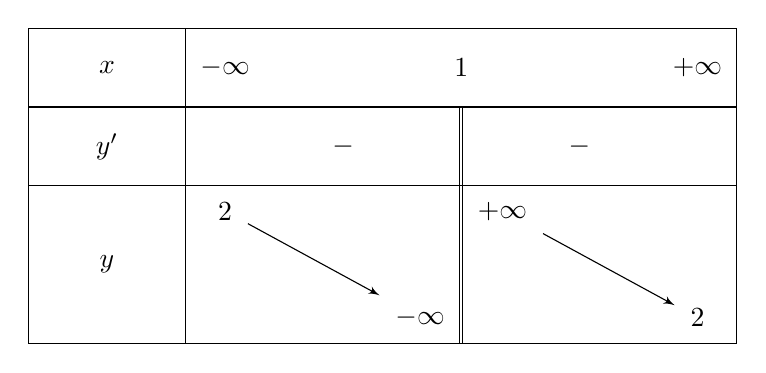
\begin{tikzpicture}
\tkzTabInit{$x$ /1, $y'$ /1, $y$ /2}{$-\infty$, $1$, $+\infty$}
\tkzTabLine{ , -, d, -, }
\tkzTabVar{+/ $2$, -D+/ $-\infty$ / $+\infty$, -/ $2$}
\end{tikzpicture}
\end{document}
